%! app: decidable languages, undecidable languages
%! outcome: Classify language, Classify decision problem, Reduction
 

Recall definition:  $A$ is  {\bf  mapping  reducible to} $B$  means there is a computable function 
$f : \Sigma^* \to \Sigma^*$ such that {\it for all} strings  $x$ in $\Sigma^*$, 
\[
x  \in  A \qquad \qquad \text{if and  only  if} \qquad \qquad f(x) \in B.
\]
Notation:  when $A$  is mapping reducible to $B$, we write $A  \leq_m B$.

{\bf Theorem} (Sipser 5.23): If $A \leq_m B$ and $A$ is undecidable, then $B$ is undecidable.
    
{\bf Halting problem}
    \[
    HALT_{TM} = \{ \langle M, w \rangle \mid \text{$M$ is a  Turing machine, $w$ is  a string, and $M$ halts on $w$} \}
    \]

We will define a computable function that witnesses the mapping reduction $A_{TM} \leq_m HALT_{TM}$.

Using Theorem 5.23, we can then conclude that $HALT_{TM}$ is undecidable.

Define $F: \Sigma^* \to \Sigma^*$ by
    \[
    F(x) =  \begin{cases}
    const_{out} \qquad &\text{if  $x \neq \langle M,w \rangle$ for any Turing machine  $M$ and string  $w$ over the alphabet of $M$} \\
    \langle M', w \rangle \qquad &  \text{if $x = \langle M, w \rangle$ for some Turing machine  $M$ and string $w$ over the alphabet of $M$.}
    \end{cases}
    \]
    where $const_{out}  =  \langle  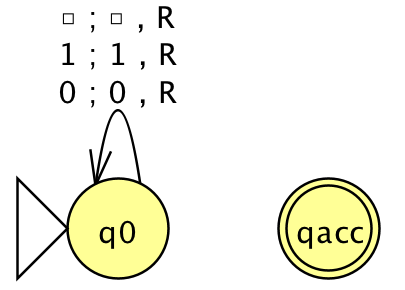
\includegraphics[width=1.5in]{../../resources/machines/Lect22TM1.png} ,  \varepsilon  \rangle$
    and  $M'$ is a Turing machine that computes like $M$ except, if the computation ever were to go to a  reject state,
    $M'$ loops instead.
    
    \vfill

    $F( \langle 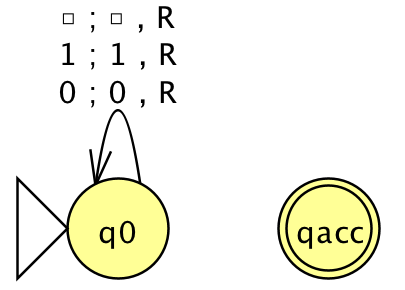
\includegraphics[width=1.5in]{../../resources/machines/Lect22TM1.png} ,  001  \rangle)$ =

    \vfill

    $F( \langle 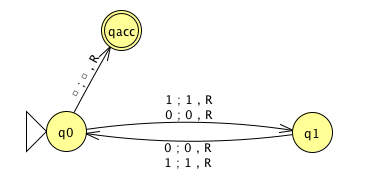
\includegraphics[width=2.5in]{../../resources/machines/Lect22TM2.png} ,  1  \rangle)$ =

    \vfill
    
    \newpage
    To use this function  to prove that $A_{TM} \leq_m HALT_{TM}$, we need  two claims:

    
    Claim (1): $F$ is computable \phantom{\hspace{2in}}
    
    \vfill

    Claim (2): for every  $x$,  $x \in  A_{TM}$ iff $F(x) \in HALT_{TM}$.  
    
    \vfill
   
    
\newpage
True or False: $\overline{A_{TM}} \leq_m \overline{HALT_{TM}}$

\vfill

True or False: $HALT_{TM} \leq_m A_{TM}$.

\vfill

\newpage